\documentclass[letterpaper,11pt]{report}

\usepackage{fullpage}
\usepackage{verbatim}
\usepackage{cite}
\usepackage{setspace}
\usepackage{fancyhdr}

%\usepackage{noReferences}
\usepackage[small]{caption}
\usepackage{graphics}
\usepackage{color}

\usepackage{hyperref}

%\usepackage{natbib}

\usepackage[dvips]{graphicx}
 % define the title
\graphicspath{ {images/} }

\setlength{\oddsidemargin}{-0.4mm} % 25 mm left margin
\setlength{\evensidemargin}{\oddsidemargin}
\setlength{\textwidth}{160mm}      % 25 mm right margin
\setlength{\topmargin}{-5.4mm}     % 20 mm top margin
\setlength{\headheight}{5mm}
\setlength{\headsep}{5mm}
\setlength{\footskip}{10mm}
\setlength{\textheight}{237mm}     % 20 mm bottom margin

\setlength{\parskip}{1ex}
\parindent 0in

\def\title{Building Management System : Scheduler and a web service to log data and control devices}

\begin{document}

\def\degreeone{B.Tech. in Computer Science and Engineering}
\def\degreetwo{B.Tech. in Electronics and Communication Engineering}
\def\btptrack{Engineering}
\def\submissiondate{November 17, 2016}
\def\supervisorone{Prof. Hemant Kumar}
\def\studentone{Divay Prakash, Amogh Vithalkar}
\def\rollnumberone{2014039, 2014134}
\def\titlelineone{Building Management System}
\def\titlelinetwo{Scheduler and a web service to log data and control devices}

\thispagestyle{empty}
\vspace{5.65in}

\begin{center}
\vspace{5.65in}
{\LARGE \bf \titlelineone{} : \titlelinetwo{}\\}
\vspace{.3in}
{\Large{Student Name: \studentone{}}}\\  
{\large{Roll Number: \rollnumberone{}}}\\
\vspace{.1in} 
\vspace{.65in}
\vspace{.65in}
{BTP report submitted in partial fulfillment of the requirements 
\\for the Degree of \degreeone{}/\\ \degreetwo{}\\}
on \submissiondate{}\\
\vspace{.65in}
\textbf{BTP Track}: \btptrack\\
\quad\\
{\textbf{BTP Advisor}\\ 
\supervisorone\\} 
\vspace{3.0in}
{Indraprastha Institute of Information Technology\\
New Delhi}
\end{center}


\newpage
\setcounter{page}{2}
\begin{center}
\textbf{\Large Student's Declaration}\label{section:declaration}
\end{center}
We hereby declare that the work presented in the report entitled \textbf{\title{}} submitted by us for the partial fulfillment of the requirements for the degree of \emph{Bachelor of Technology} in \emph{Computer Science \& Engineering} and \emph{Bachelor of Technology} in \emph{Electronics and Communication \& Engineering} respectively at Indraprastha Institute of Information Technology, Delhi, is an authentic record of our work carried out under guidance of \textbf{Prof. Hemant Kumar}. Due acknowledgements have  been given in the report to all material used. This work has not been submitted anywhere else for the reward of any other degree.\\
\vspace{0.5in}

\textbf{..............................}\hfill
\textbf{ Place \& Date: .............................}\\
\textbf{Divay Prakash, Amogh Vithalkar}

\vspace{3in}
\begin{center}
\textbf{\Large Certificate} \label{section:certificate}
\end{center}
This is to certify that the above statement made by the candidate is correct to the best of my knowledge.\\
\vspace{0.4in}

\textbf{..............................}\hfill
\textbf{ Place \& Date: .............................}\\
\textbf{Prof. Hemant Kumar}

\pagebreak

\begin{abstract}

The building management HVAC(heating, ventilation and air conditioning) system for Phase II is designed to take care (and advantage) of diversity of use. Instead of using large AHUs(Air Handling Units), we will have individual units in faculty rooms, labs, and other spaces. This would allow us to condition air of the spaces that are occupied and the system would be able to maintain desired temperature more closely. The disadvantage of this approach is higher capital cost and a larger I/O points for BMS but the running cost will be saved. In this project we are developing a scheduler hosted on a web server to control the AC’s valves connected through RaspberryPi and Arduino.

\vspace{2.15in}
Keywords: building management system, scheduler, web server 
\end{abstract}

\newpage
\section*{Acknowledgments}\label{section:acknowledgments}
\pagestyle{plain}
\pagenumbering{roman}

I would like to express my sincere gratitude to my supervisor Prof. Hemant Kumar for providing his invaluable guidance, comments and suggestions throughout the course of the project. 

\vspace{2in}
%\section*{Work Distribution}
%% explain chapterwise when the reported work has been done.

\newpage

\tableofcontents

\chapter{Introduction}\label{chapter:introduction}
\pagenumbering{arabic}
\setcounter{page}{1}
\onehalfspacing
\section{BMS for phase I}
HVAC for the Phase I buildings (Academic, Lecture halls and library building) used large floor mounted AHUs to condition large spaces except lecture halls which were served by CSUs (ceiling suspended units). Library building has one AHU per floor feeding all the labs and rooms. The academic building has 4 AHUs (two serving A wing and the other two wing B). The AHU of wing A serves 4 th and 5 th floors while the other 1st , 2nd and 3rd . Hostels have one FCU per room. The large AHUs of the academic block control volume of cold air by reducing the fan speed using VFD drives. As the area per AHU is large and the need very diverse (labs with varying number of occupants and equipment vs faculty rooms), the HVAC system is not very xxxx and energy efficient. The HVAC system has a very basic centralized control system that can set temperature to be achieved in each one the AHUs or CSUs. It also allows switching on/ off, monitoring parameters etc centrally. Other than AHUs/CSUs it can display status and parameters of chillers, cooling towers and hot water generator.
\par
In BMS/ HVAC terminology each point that is controlled or read is an I/O point and an I/O summary is prepared for any BMS installation to estimate the cost. The I/O points are of 4 types –  digital input, digital output, analog input and analog output. In phase I, we had chosen to only include I/O that either needed to be controlled or the I/O that were to be sensed and used for controlling to contain cost. The system was provided by Trane.
\par
Later a parallel system was implemented by a research group led by Dr Amarjeet Singh. This group installed wireless temperature sensors (13) and Ethernet based power meters (500) all over the campus to optimize HVAC and energy use based on data collected.
\pagebreak
\section{BMS for phase II}
The HVAC for Phase II is designed to take care (and advantage) of diversity of use. So instead of large AHUs, we will have individual units in faculty rooms, labs, and other spaces. This would allow us to condition air of the spaces that are occupied and the system would be able to maintain desired temperature more closely. The disadvantage of this approach is higher capital cost and a larger I/O points for BMS but the running cost will be saved.

\newpage
\chapter{Architecture}\label{chapter:architecture}
\onehalfspacing
\begin{figure}[h]
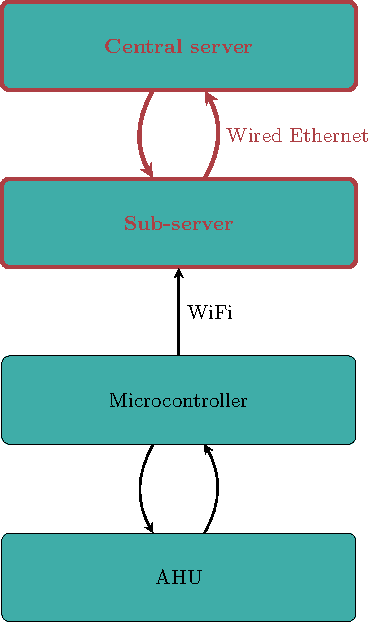
\includegraphics[width=3cm, height=7cm]{arch}
\centering
\captionsetup{justification=centering}
\caption{Block diagram of the building management system project}
\label{fig:arch}
\end{figure}
The BMS (Building Management System)/ HVAC (Heating, Ventilation and Air-Conditioning) system, is structured in the manner described by figure \ref{fig:arch}. At the lowest level is the AHU (Air Handling Unit), which performs the actual cooling/heating functionality of the system. It is controlled by the microcontroller. The microcontroller monitors various system parameters and accordingly runs the AHU. It is in turn controlled by a sub-server unit, which is responsible for logging data and passing control instructions to the microcontroller unit according to policies set by the central server. The highlighted sections in figure \ref{fig:arch} are the modules that were worked upon over the course of this project. In addition, code documentation for the entire stack was also written.

\newpage
\chapter{Design}\label{chapter:Design}
\onehalfspacing
\section{Overview}
\begin{figure}[h]
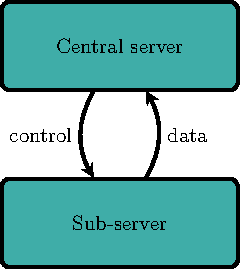
\includegraphics[width=4cm, height=4.5cm]{des}
\centering
\captionsetup{justification=centering}
\caption{Higher level control modules of the building management system}
\label{fig:des}
\end{figure}
The higher level control of the building management system is carried out by the central server in conjunction with various sub-server units managing their own group of microcontroller devices. The details of the central server and the sub-servers are given in the following sections.
\section{Central server}
The central server of the system is a software implementation only. There are no specific hardware requirements for the same. The server is implemented in such a manner so as to be able to provide interfaces to both the sub-server devices using a REST API and also to system administrators by way of a GUI. This can be broken down into two main modules, the frontend and the backend. Both of these modules were built over the course of this project.
\subsection{Frontend}
The frontend of the central server consists of a hierarchy of web pages created using HTML/\newline CSS/JavaScript/jQuery and the Bootstrap framework. This provides the GUI which can be used by system administrators for overall analysis/control of the system.
\subsection{Backend}
The backend of the central server consists of a web application created using the Python web framework Django. The system used MySQL as the database management system.
\section{Sub-server}
The sub-servers are individual Raspberry Pi units running a Linux OS distribution. These devices are connected to the network using a wired Ethernet connection and each unit manages upto 20 AVR microcontroller units. The Raspberry Pi devices host a web server which provides various functionalities. Over the course of this project, the web server was ported from a \verb|BaseHTTPServer| to a Django-based server, both coded in Python.

\newpage
\chapter{Implementation}\label{chapter:Implementation}
\onehalfspacing
\section{Central server}
\subsection{Description}
The central server is a Django web application which uses a MySQL DBMS.\\ \\
{\huge{**** TODO ****}}
\subsection{Functionality}
{\huge{**** TODO ****}}
\section{Sub-server}
\subsection{Description}
The Raspberry Pi units serving as sub-servers run a Django based web application which serves a REST API. This is utilised by both the microcontrollers and the central server which communicate with the device using HTTP messages. In addition, the sub-server device also functions as a client in some cases. This is further explained in the next section.
\subsection{Functionality}
\subsubsection{For microcontroller}
All communication taking place between sub-server devices and the microcontrollers follows the client-server model. However, the server (Rapberry Pi device) cannot initiate a message send to the client (microcontroller) without a prior request from the client. Due to memory and threading constraints at the microcontroller end, interrupts have not been used. Thus all communication is initiated by the client device. 
\begin{itemize}
    \item Data logging - The sub-server device provides a REST API method for microcontroller devices to log data. The microcontroller devices makes an HTTP POST request to the Raspberry Pi sub-server, which processes the attached data and stores it in the database. This data is stored in a MySQL database using microcontroller MAC addresses and the HTTP message timestamp as keys. Thereafter, the sub-server sends a confirmation message back to the client.
    \item Fetching commands - The microcontroller devices also fetch commands from the sub-server units. For this purpose, the microcontroller makes an HTTP GET request to the sub-server. The sub-server extracts the microcontroller's MAC address from the request and queries its database for any pending commands to be sent to that device. If found, it returns the same in the HTTP response to the client, else an empty response is sent.
\end{itemize}
\subsubsection{For central server}
In case of the communication with the central server, the model followed is again client-server model. However, both thee sub-server and central server can initiate message sending.
\begin{itemize}
    \item Receive commands - The sub-server device acts as a client for this method, used by the central server to transmit commands to the sub-server using HTTP messages.
    \item Send data
    \begin{itemize}
        \item With prior request - This method is followed if the central server requests data logs from the sub-server using an HTTP GET message as-and-when required.
        \item With no prior request - The Raspberry Pi device uses an SD card to store data persistently. To ensure longevity of the system, it is essential to keep the number of read/write cycles on the card to a minimum. Thus data logs are stored in primary memory. While this solves the SD card issue, it creates another as main system memory is being taken up by static data. To resolve this issue, the Raspberry Pi device dumps the data logs to the central server using HTTP POST messages at a fixed time interval. This enables the deletion of the files at sub-server end, freeing up valuable memory resources.
    \end{itemize}
\end{itemize}

%\newpage
%\bibliographystyle{these}
\bibliographystyle{acm}
%\bibliographystyle{elsart-harv}
%\newpage
%\section{References}
%\bibliography{Library}
\bibliography{sample}

%\chapter*{Appendix}\label{chapter:appendix} 

\end{document}
